\documentclass{article}
\usepackage[utf8]{inputenc}
\usepackage{graphicx}
\usepackage[margin=1in]{geometry}
\usepackage[dvipsnames]{xcolor}
\usepackage{url}
\usepackage{hyperref}
\usepackage[numbers]{natbib} % for numeric references

\begin{document}

\begin{titlepage}
    \begin{center}
        
\includegraphics[width=3cm]{figures/MSP-logo.jpg} 
        \vspace{1cm}
        
        \textbf{\LARGE Individual Variation in Humboldt Penguins' 
        Speed}\\
        
        
        
        \vspace{1.5cm}
        
        \textbf{\Large Juana Garcia Masi (ID6377648)}
        
        \vfill
        
        \large Date: \today
        
    \end{center}
\end{titlepage}

\newpage

\section*{Introduction}
Humboldt penguins live across the South American coast, from Peru to southern Chile. These mostly sedentary creatures stay close to their colonies but can swim 20–35 km away in search of food~\cite{source}. Tracking wildlife movements helps understand their biology, and identify and reduce disturbances, such as human activity. It is also important to take into consideration individual variation, since a small sample may not represent the full range of behaviours within a population. This report explores whether individual Humboldt penguins differ in their hourly movement speed and how much variation is explained by individual identity. To answer this, a one-way ANOVA was applied to test $H_0$: all penguins have the same mean hourly speed, against $H_1$: at least one penguin's mean speed differs.

\section*{Data sample}
The dataset used included one file with the tracked positions of 21 Humboldt penguins in Isla Choros, Chile, during the autumn and spring breeding seasons of 2022~\cite{dataset}. Each event ID shows their longitude and latitude positions on an hourly basis and their local ID. The relevant columns used in this analysis were:
\begin{itemize}
    \item Location-long: Longitude coordinate
    \item Location-lat: Latitude coordinate
    \item Timestamp: Time of the event
    \item Individual-local-identifier: Individual identity for each penguin
\end{itemize}

\indent The dataset required cleaning, with one duplicate track removed, leaving 20 penguins in total.
To find the penguins’ speed, the distance between each penguin's consecutive hourly positions was calculated using the haversine formula, then divided by time to get speed in kilometers per hour: 
\begin{equation}
a = \sin^2\left(\frac{\Delta \phi}{2}\right)
+ \cos(\phi_1)\cos(\phi_2)
\sin^2\left(\frac{\Delta \lambda}{2}\right)
\end{equation}

\begin{equation}
d = 2R \arcsin\left(\sqrt{a}\right)
\end{equation}

\indent Where latitude ($\phi$) and longitude ($\lambda$) are in radians, and R is 6371 km, the mean radius of the Earth. This gave the displacement per hour, with only the steps with one hour between fixes kept, leaving 329 hourly speed values.

\section*{Results and discussion}
Each penguin’s mean speed was calculated, showing large variability within individuals, with standard deviation often comparable to the mean (Figure 1). To test whether individuals differ, the one-way ANOVA test was applied. Its F-statistic is the variance between penguin means relative to the variance within penguins.
\begin{equation}
    F =\frac{\mbox{MS between}}
    {\mbox{MS within}}
\end{equation}

The results show F(19,309)= 5.39, p \(<\) 0.001, with the mean speeds ranging from 0.16 to 3.71 km/h. Therefore, between penguin differences are larger than expected by chance. To quantify how much the individual identity explained the variance, the effect size was calculated:
\begin{equation}
    \eta^2 = \frac{F \cdot df_{between}}{F \cdot df_{between} + df_{within}}
\end{equation}
Individual identity explained about 25\%\ of the observed variance in speed ($\eta^2$= 0.25), so most of the variation happened within individuals. Therefore, the null hypothesis is rejected.

\begin{figure}[h]
    \centering
    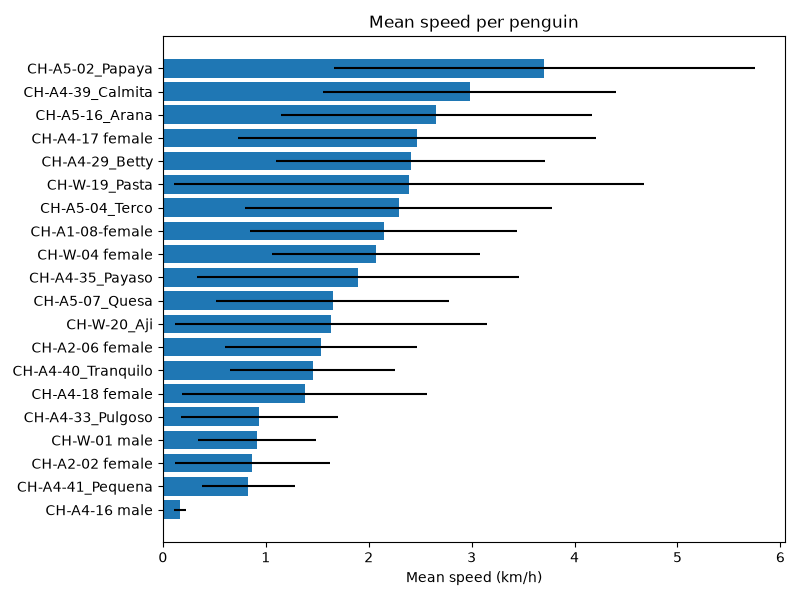
\includegraphics[width=0.6\linewidth]{Figure 1.png}
    \caption{Mean speed of each penguin, with each error bar representing the standard deviation.}
    \label{fig:placeholder}
\end{figure}
\begin{figure}[h]
    \centering
    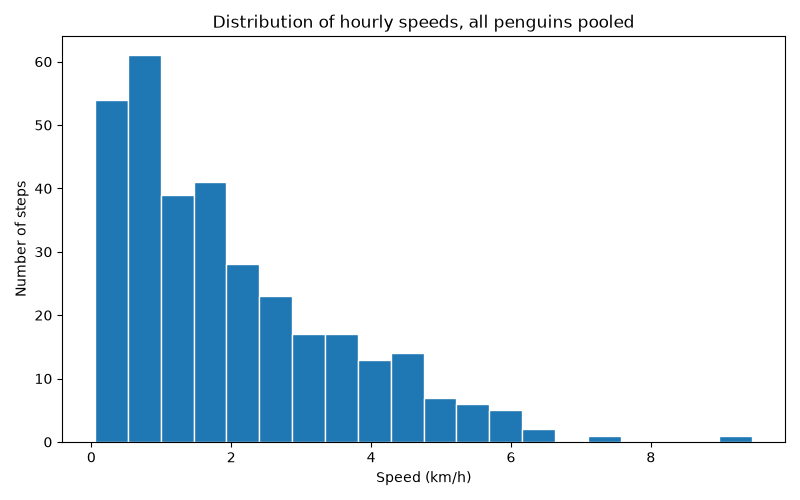
\includegraphics[width=0.5\linewidth]{Figure 2.png}
    \caption{Distribution of hourly speeds pooled together.}
    \label{fig:placeholder}
\end{figure}

\indent There are some limitations to take into account, such as the speed being right-skewed (Figure 2) and showing a lot of variability, so the ANOVA assumptions are not fully met. In addition, the speed reflects hourly displacement, not path length, which could underestimate their actual speeds. Consecutive hourly steps from the same penguin are also unlikely to be independent, so the p-value may be too optimistic.

\indent In conclusion, individual identity explains about a quarter of the variation in speed, suggesting that individual variation should be taken into account when sampling a population.

\begin{thebibliography}{9}

\bibitem{source}
Humboldt penguin \textit{Spheniscus humboldti} species factsheet. (n.d.). 
BirdLife DataZone. 
\url{https://datazone.birdlife.org/species/factsheet/humboldt-penguin-spheniscus-humboldti}

\bibitem{dataset}
Bastías, I., Mattern, T., Ellenberg, U., Daigre, M., Simeone, A. (2026). Data from: Spatio-temporal overlap between purse seine fisheries and Humboldt penguin feeding areas in northern Chile [Dataset]. In Movebank. \url{https://doi.org/10.5441/001/1.725}

\end{thebibliography}
\end{document}